\documentclass[11pt,a4paper]{article}
\usepackage{a4wide}
\usepackage{enumerate}
\usepackage{enumitem}
\usepackage{pcptex}
\usepackage{xspace}
\usepackage[toc,page]{appendix}
\usepackage{algorithm}
\usepackage[noend]{algpseudocode}
\usepackage{hyperref}
\usepackage{xcolor}
\usepackage{tikz}
\usepackage{pgfplots}

\renewcommand{\arraystretch}{1.2}

\definecolor{links}{HTML}{2A1B81}
\hypersetup{colorlinks,linkcolor=,urlcolor=links}

\makeatletter
\def\BState{\State\hskip-\ALG@thistlm}
\makeatother

\setlength{\parindent}{0pt}


\begin{document}

\pptitle{A High Performance Implementation of the 2D nBody Gravitational problem: Barnes-Hut versus Brute-Force}

\ppintro{Gael Lederrey}{EPFL-CSE}{/}{Only PI}{\today}{June 15, 2016}{Deneb}{NBODY-BHVSBF}


\ppabstract{The nBody problem has been well studied by many scientists in many different fields such as atomistic simulation or astrophysics. In this project, we present the implementation of the Barnes-Hut algorithm. A shared memory version using the MPI library will also be presented. A benchmark comparison is done with the Brute-Force algorithm, serial and parallel versions.}

\section{Scientific Background}
\subsection{Algorithms}

The nBody problem covers the whole scale of science from the subatomic particles to the gigantic galaxies. It is a problem that has been studied a lot and new papers are still being published about this problem. In order to solve this problem, it exists a really easy solution called Brute-Force. This method is really simple to implement. It consists in looping on all the objects and inside this loop, it loops again on all the objects:
\begin{algorithm}
\caption{Brute-Force}\label{bf}
\begin{algorithmic}[1]
\State $n$ = Number of bodies
\State Initialize $n$ objects
\While {$t < t_{end}$}
\For {$i = 1 \textit{ to } n$} 
\For {$j = 1 \textit{ to } n$}
\State Apply forces from body $j$ on body $i$
\EndFor
\EndFor
\For {$k = 1 \textit{ to } n$}
\State Update the body $k$
\EndFor
\EndWhile
\end{algorithmic}
\end{algorithm}

We can clearly see that the loop to calculate all the forces is in $\mathcal{O}(n^2)$. Updating the bodies will take only $\mathcal{O}(n)$ time. But most of the time will be spent in the calculation of the forces. For a very large number of bodies this algorithm will be very slow. Therefore another algorithm can be used: Barnes-Hut.

The Barnes-Hut algorithm is easy to understand. First, it consists in building a quadtree and place each body in the leaves of this tree. Each parent node will store the center of mass of its leaves. Then, we can apply the forces for each body. Instead of calculating all the forces between the current body and all the other bodies, it uses the center of the mass of multiple bodies if there are far away from the current body. The pseudo-code is given below:
\begin{algorithm}
\caption{Barnes-Hut}\label{bh}
\begin{algorithmic}[1]
\State $n$ = Number of bodies
\State Initialize $n$ objects
\While {$t < t_{end}$}
\For {$i = 1 \textit{ to } n$} 
\State	Add body $i$ in the tree
\EndFor
\For {$j = 1 \textit{ to } n$} 
\State	Calculate all the forces applied to bod $j$.
\EndFor	
\For {$k = 1 \textit{ to } n$}
\State Update the body $k$
\EndFor
\EndWhile
\end{algorithmic}
\end{algorithm}

Adding a body in the tree takes $\mathcal{O}(\log n)$ time (height of the tree). Therefore, adding all the bodies will take $\mathcal{O}(n\log n)$ time. The calculation of the forces will take $\mathcal{O}(n) \times \mathcal{O}(\log n) = \mathcal{O}(n\log n)$ time. And finally, updating the bodies will take $\mathcal{O}(n)$ time. Therefore, this algorithm will take $\mathcal{O}(n\log n)$ time which is much faster than the Brute-Force algorithm for a high number of bodies.
\\\\
For both algorithms, the communication between the process is proportional to the number of bodies. Therefore, we can say that communication is in $\mathcal{O}(n)$ time.

\subsection{Gravitation} 

In order to take a real test case for the nBody problem, we choose the Gravitational nBody problems. The forces are given by:
\begin{equation}
\vec{F}_{1\rightarrow 2} = G\cdot\frac{m_1m_2(\vec{x}_2-\vec{x}_1)}{\Vert \vec{x}_2-\vec{x}_1\Vert^3}
\end{equation}
where $G$ is the gravitational constant and is equal to $6.674 \cdot 10^{-11}~[Nm^2kg^{-2}]$. As we can see with this equation, the forces decreases proportionally to $1/r^2$, $r$ being the distance between two bodies. This allows the center of the mass approximation in the Barnes-Hut algorithm. Indeed, if two bodies are close to each other and far away from a third body. The two forces of these bodies on the third one will be almost the same as the force of the center of the mass of the two far bodies.

\section{Project Description}

In this project we want to implement a high performance version of the Barnes-Hut algorithm in C++. A simple version of the Brute-Force algorithm will also be implemented in order to be used as a benchmark for the Barnes-Hut algorithm. At the end, four different codes will be produced:
\begin{itemize}
\item Serial version of the Brute-Force algorithm
\item Shared memory version, using MPI~\cite{mpi}, of the Brute-Force algorithm
\item Serial version of the Barnes-Hut algorithm
\item Shared memory version, using MPI~\cite{mpi}, of the Barnes-Hut algorithm
\end{itemize}
The three first codes will be used as benchmark for the shared memory version of the Barnes-Hut algorithm. Indeed, to prove that this version is the fastest, we need to make sure it overcomes the Brute-Force algorithm. 
\\\\
For the two shared memory codes, we determine the Amdahl's law. We will then compare the Strong scaling and the weak scaling. For the Shared memory version of the Barnes-Hut algorithm, we will study the effect on the Load-Balancing on the processors. 

\section{Implementations}

These four applications are implemented in C++~\cite{c++}. As it was said in the previous section, the shared memory versions are using the MPI library~\cite{mpi}. Everything has been compiled using \verb+gcc+ version 4.8.4. The code have been debugged using the general debugged \verb+gdb+. And \verb+valgrind+ has been used to remove all the memory leaks. 

\subsection{Optimizations}

For each of the codes, we compile it once without using any optimization flags and once with the following two flags: \verb+-Ofast+ and \verb+-ftree-vectorize+. The non-optimized version will not be used. It was just for testing purpose.

\subsubsection{Brute-Force}

Not much efforts were put onto the optimization of the Brute-Force algorithm since it exists only for a benchmark purpose. For the MPI version of the code, the first (outer) loop is divided into the number of processes. The second (inner) loop is still on the $n$ bodies. After the update of the local bodies, everything is sent back to the master process to update the vector of all the bodies. It also redistribute equally the number of local bodies to all the processes to keep a good load-balancing.

\subsubsection{Barnes-Hut}

For the Barnes-Hut algorithm, loop reordering and vectorization is not useful since it only uses pointers. The following is only a supposition since the code has not been written yet. We will try to do the construction of the tree in parallel on all the processes. We will also try to make the calculation of the forces parallel. After the update of all the bodies, everything will be send to the master process in order to recreate the vector of all the bodies. We will also try to find a metric to tell when it is good to recreate the quadtree. Indeed, the creation of the tree can take some time, so it is good if it does not have to be recreated at each iteration.

\section{Amdahl's law}

The Amdahl's law is given by:
\begin{equation}
S_{p} = \frac{1}{\alpha + \frac{1-\alpha}{p}}
\end{equation}
where $S_{p}$ is the theoretical speedup, $1-\alpha$ is the parallelizable part of the code and $p$ is the number of processors. Ideally, we should have $S_p = p$. But this does not happen in reality.

\subsection{Brute-Force}

In the Brute-Force algorithm, everything can be parallelized except the loading of the data at the beginning and the communication between the process. Since this algorithm is in $\mathcal{O}(n^2)$, the loading time at the beginning will be negligible compared to the time taken for the calculation of the forces. Therefore, the speedup will be really close to the perfect speedup, {\it i.e.} $S_p = p$.

\subsection{Barnes-Hut}

In the Barnes-Hut algorithm, we can also parallelize everything except the loading of the data and the communication. But since this algorithm is in $\mathcal{O}(n\log n)$, the fraction of serial code will be much higher compared to the Brute-Force algorithm. Therefore, we can except a smaller speedup.

\subsection{Results}

Table \ref{tab:amdahl} presents different times taken by the code for the Brute-Force and the Barnes-Hut algorithms. $t_L$ corresponds to the loading time, $\overline{t}_{it}$ is the mean iteration time and  $\overline{t}_{com}$ is the mean communication time. The total time taken by the algorithm will be:
\begin{equation}
t_{tot,q} = t_L + q\cdot(\overline{t}_{it} + \overline{t}_{com})
\end{equation}
where $q$ is the number of iterations. Therefore, we can calculate the fraction of serial code for a given number of iterations:
\begin{equation}
\alpha_q = \frac{t_L + q\cdot \overline{t}_{com}}{t_{tot,q}}
\end{equation}
The fraction $\alpha_q$ for $q=100$ and $q=1000$ is given in the table \ref{tab:amdahl}. For the moment, the communication time is not taken into account because the MPI code for the Barnes-Hut algorithm has not been done. Therefore, we can only take into account the loading time. This table will be done again and the Amdahl's law will be corrected after the implementation of the MPI for the Barnes-Hut algorithm.
\\
Finally, with this fraction $\alpha_q$, we can plot the Amdahl's law as it is given in the figure \ref{fig:amdahl}. We can clearly see that the theoretical speedup for the Barnes-Hut algorithm is much lower than for the Brute-Force algorithm. 

\newpage
\begin{table}[h]
\centering
\begin{tabular}{|c||c|c|c|c||c|c|}
\hline
Algorithm & $n$ & $t_L~[s]$ & $\overline{t}_{it}~[s]$ & $\overline{t}_{com}~[s]$ & $\alpha_{100}$ & $\alpha_{1000}$ \\
\hline \hline
\multirow{3}{*}{Brute-Force} & $10^4$ & 0.0588 & 1.300 & / & $4.52\cdot10^{-4}$ & $4.52\cdot10^{-5}$ \\ \cline{2-7}
& $10^5$ & 0.554 & 130.1 & / & $4.26\cdot10^{-5}$ & $4.26\cdot10^{-6}$ \\ \cline{2-7}
& $10^6$ & 4.709 & 13234.7 & / & $3.56\cdot10^{-6}$ & $3.56\cdot10^{-7}$ \\ \hline
\multirow{3}{*}{Barnes-Hut} & $10^4$ & 0.121 & 0.0361 & / & $3.34\cdot10^{-2}$ & $3.34\cdot10^{-3}$ \\ \cline{2-7}
& $10^5$ & 0.498 & 0.539 & / & $9.23\cdot10^{-3}$ & $9.23\cdot10^{-4}$ \\ \cline{2-7}
& $10^6$ & 4.730 & 5.921 & / & $7.99\cdot10^{-3}$ & $7.99\cdot10^{-4}$ \\ \hline
\end{tabular}
   \caption{Times used to calculate the serial part of the code for the Amdahl's law.}
   \label{tab:amdahl}  
\end{table}

\begin{figure}[H]
\centering
% This file was created by matlab2tikz.
% Minimal pgfplots version: 1.3
%
%The latest updates can be retrieved from
%  http://www.mathworks.com/matlabcentral/fileexchange/22022-matlab2tikz
%where you can also make suggestions and rate matlab2tikz.
%
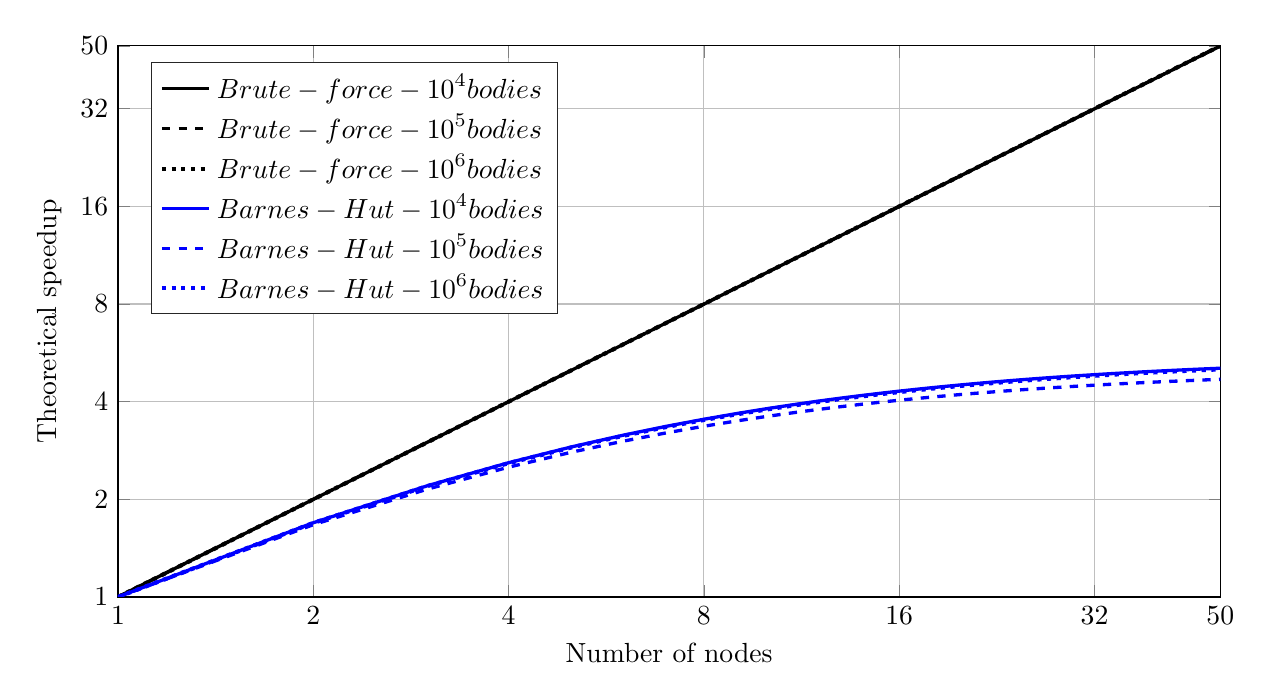
\begin{tikzpicture}

\begin{axis}[%
width=14cm,
height=7cm,
at={(0.769167in,0.484687in)},
scale only axis,
xmode=log,
xmin=1,
xmax=50,
xtick={1,2,4, 8, 16, 32, 50},
xticklabels={{1},{2},{4},{8},{16},{32}, {50}},
xminorticks=true,
xlabel={Number of nodes},
xmajorgrids,
xminorgrids,
ymode=log,
ymin=1,
ymax=50,
ytick={1,2,4, 8, 16, 32, 50},
yticklabels={{1},{2},{4},{8},{16},{32}, {50}},
yminorticks=true,
ylabel={Theoretical speedup},
ymajorgrids,
yminorgrids,
legend style={at={(0.03,0.97)},anchor=north west,legend cell align=left,align=left,draw=white!15!black}
]
\addplot [color=black,solid,line width=1.2pt]
  table[row sep=crcr]{%
1	1\\
2	1.99994667610975\\
3	2.99984003259429\\
4	3.99968007371821\\
5	4.99946680374565\\
6	5.99920022694027\\
7	6.99888034756531\\
8	7.99850716988353\\
9	8.99808069815725\\
10	9.99760093664832\\
11	10.9970678896182\\
12	11.9964815613277\\
13	12.9958419560375\\
14	13.9951490780075\\
15	14.9944029314973\\
16	15.9936035207661\\
17	16.9927508500726\\
18	17.9918449236749\\
19	18.9908857458309\\
20	19.9898733207979\\
21	20.9888076528327\\
22	21.9876887461918\\
23	22.986516605131\\
24	23.985291233906\\
25	24.9840126367717\\
26	25.9826808179827\\
27	26.9812957817933\\
28	27.979857532457\\
29	28.9783660742272\\
30	29.9768214113565\\
31	30.9752235480974\\
32	31.9735724887018\\
33	32.9718682374209\\
34	33.9701107985058\\
35	34.9683001762071\\
36	35.9664363747747\\
37	36.9645193984584\\
38	37.9625492515072\\
39	38.9605259381699\\
40	39.9584494626946\\
41	40.9563198293293\\
42	41.9541370423213\\
43	42.9519011059174\\
44	43.9496120243642\\
45	44.9472698019075\\
46	45.944874442793\\
47	46.9424259512657\\
48	47.9399243315702\\
49	48.9373695879508\\
50	49.9347617246512\\
};
\addlegendentry{$\text{Brute-force - 10}^\text{4}\text{ bodies}$};

\addplot [color=black,dashed,line width=1.2pt]
  table[row sep=crcr]{%
1	1\\
2	1.99999718001251\\
3	2.99999154004945\\
4	3.99998308012275\\
5	4.99997180024435\\
6	5.99995770042617\\
7	6.99994078068014\\
8	7.99992104101818\\
9	8.99989848145223\\
10	9.99987310199421\\
11	10.9998449026561\\
12	11.9998138834497\\
13	12.999780044387\\
14	13.99974338548\\
15	14.9997039067406\\
16	15.9996616081806\\
17	16.9996164898121\\
18	17.999568551647\\
19	18.9995177936971\\
20	19.9994642159744\\
21	20.9994078184909\\
22	21.9993486012584\\
23	22.999286564289\\
24	23.9992217075944\\
25	24.9991540311867\\
26	25.9990835350778\\
27	26.9990102192795\\
28	27.9989340838039\\
29	28.9988551286628\\
30	29.9987733538682\\
31	30.9986887594321\\
32	31.9986013453662\\
33	32.9985111116826\\
34	33.9984180583932\\
35	34.9983221855099\\
36	35.9982234930447\\
37	36.9981219810094\\
38	37.998017649416\\
39	38.9979104982764\\
40	39.9978005276025\\
41	40.9976877374064\\
42	41.9975721276998\\
43	42.9974536984947\\
44	43.9973324498031\\
45	44.9972083816368\\
46	45.9970814940079\\
47	46.9969517869282\\
48	47.9968192604096\\
49	48.9966839144641\\
50	49.9965457491035\\
};
\addlegendentry{$\text{Brute-force - 10}^\text{5}\text{ bodies}$};

\addplot [color=black,dotted,line width=1.5pt]
  table[row sep=crcr]{%
1	1\\
2	1.9999992455067\\
3	2.99999773652095\\
4	3.99999547304362\\
5	4.99999245507554\\
6	5.99998868261758\\
7	6.99998415567059\\
8	7.99997887423542\\
9	8.99997283831293\\
10	9.99996604790397\\
11	10.9999585030094\\
12	11.9999502036301\\
13	12.9999411497668\\
14	13.9999313414205\\
15	14.999920778592\\
16	15.9999094612822\\
17	16.9998973894918\\
18	17.9998845632219\\
19	18.9998709824731\\
20	19.9998566472464\\
21	20.9998415575427\\
22	21.9998257133627\\
23	22.9998091147073\\
24	23.9997917615775\\
25	24.9997736539739\\
26	25.9997547918976\\
27	26.9997351753493\\
28	27.9997148043299\\
29	28.9996936788403\\
30	29.9996717988813\\
31	30.9996491644537\\
32	31.9996257755585\\
33	32.9996016321964\\
34	33.9995767343683\\
35	34.9995510820752\\
36	35.9995246753177\\
37	36.9994975140969\\
38	37.9994695984135\\
39	38.9994409282683\\
40	39.9994115036624\\
41	40.9993813245964\\
42	41.9993503910713\\
43	42.9993187030879\\
44	43.999286260647\\
45	44.9992530637496\\
46	45.9992191123964\\
47	46.9991844065884\\
48	47.9991489463263\\
49	48.9991127316111\\
50	49.9990757624435\\
};
\addlegendentry{$\text{Brute-force - 10}^\text{6}\text{ bodies}$};

\addplot [color=blue,solid,line width=1.2pt]
  table[row sep=crcr]{%
1	1\\
2	1.6937899510075\\
3	2.20334216965291\\
4	2.59344192354659\\
5	2.90168652023547\\
6	3.15139327484974\\
7	3.3577912616699\\
8	3.53124848721009\\
9	3.67906809928399\\
10	3.80654294649019\\
11	3.91760274810478\\
12	4.01522637737897\\
13	4.10171304425647\\
14	4.17886567627005\\
15	4.24811796544492\\
16	4.31062428772729\\
17	4.36732456528899\\
18	4.41899185637153\\
19	4.46626781077842\\
20	4.50968945352666\\
21	4.54970967422904\\
22	4.58671308287264\\
23	4.62102841010838\\
24	4.6529382998322\\
25	4.68268711217689\\
26	4.71048719307112\\
27	4.73652395078827\\
28	4.76095999619283\\
29	4.7839385421459\\
30	4.80558621224844\\
31	4.8260153752877\\
32	4.84532609626958\\
33	4.86360777554752\\
34	4.88094053271128\\
35	4.89739638043212\\
36	4.91304022454\\
37	4.92793071962079\\
38	4.94212100391271\\
39	4.95565933291098\\
40	4.96858962760298\\
41	4.98095195045862\\
42	4.9927829200442\\
43	5.00411607329853\\
44	5.01498218302057\\
45	5.02540953689811\\
46	5.03542418340513\\
47	5.0450501490685\\
48	5.05430963091904\\
49	5.06322316737192\\
50	5.07180979030545\\
};
\addlegendentry{$\text{Barnes-Hut - 10}^\text{4}\text{ bodies}$};

\addplot [color=blue,dashed,line width=1.2pt]
  table[row sep=crcr]{%
1	1\\
2	1.67045595392877\\
3	2.15122262669296\\
4	2.51282529355071\\
5	2.7946831136722\\
6	3.0205556205969\\
7	3.2056163683254\\
8	3.36000997234063\\
9	3.49077610601366\\
10	3.60295297064327\\
11	3.70024139831853\\
12	3.78542098544317\\
13	3.86061994924348\\
14	3.92749537556431\\
15	3.98735675224598\\
16	4.04125256988969\\
17	4.09003226056965\\
18	4.13439129697756\\
19	4.17490456175802\\
20	4.21205139842249\\
21	4.24623466659004\\
22	4.27779541150231\\
23	4.30702428195494\\
24	4.33417050754315\\
25	4.35944902295441\\
26	4.38304617067176\\
27	4.40512430237917\\
28	4.42582551945939\\
29	4.44527473482025\\
30	4.46358219549278\\
31	4.48084557363471\\
32	4.49715170969999\\
33	4.5125780734583\\
34	4.52719399474528\\
35	4.541061705201\\
36	4.55423722401665\\
37	4.5667711142776\\
38	4.57870913143453\\
39	4.59009278143526\\
40	4.60095980286681\\
41	4.61134458491023\\
42	4.62127853086129\\
43	4.63079037531225\\
44	4.63990646174279\\
45	4.64865098616808\\
46	4.6570462115893\\
47	4.6651126572488\\
48	4.67286926607704\\
49	4.68033355320799\\
50	4.68752173801374\\
};
\addlegendentry{$\text{Barnes-Hut - 10}^\text{5}\text{ bodies}$};

\addplot [color=blue,dotted,line width=1.5pt]
  table[row sep=crcr]{%
1	1\\
2	1.691421267001\\
3	2.19800335525537\\
4	2.58512724431123\\
5	2.89059086663529\\
6	3.1377672908751\\
7	3.34188660133655\\
8	3.51329796445007\\
9	3.65927987990264\\
10	3.78510039650046\\
11	3.89466642690251\\
12	3.9909366804081\\
13	4.07619286756916\\
14	4.15222285768443\\
15	4.22044742612696\\
16	4.28200987107316\\
17	4.33784059917366\\
18	4.38870447407415\\
19	4.4352360663391\\
20	4.4779662641571\\
21	4.51734261811561\\
22	4.55374507636363\\
23	4.58749828431542\\
24	4.61888129324529\\
25	4.64813529300237\\
26	4.67546982260366\\
27	4.70106779715546\\
28	4.72508960619414\\
29	4.74767647758651\\
30	4.76895325608716\\
31	4.78903071203335\\
32	4.80800747033416\\
33	4.82597163066769\\
34	4.84300213505739\\
35	4.85916992761708\\
36	4.87453894240263\\
37	4.88916694837746\\
38	4.90310627503627\\
39	4.91640443789987\\
40	4.92910467963817\\
41	4.94124643980696\\
42	4.95286576394922\\
43	4.96399566100014\\
44	4.97466641645997\\
45	4.98490586759234\\
46	4.99473964591353\\
47	5.00419139142041\\
48	5.01328294232639\\
49	5.02203450351125\\
50	5.03046479641954\\
};
\addlegendentry{$\text{Barnes-Hut - 10}^\text{6}\text{ bodies}$};

\end{axis}
\end{tikzpicture}%
\caption{\label{fig:amdahl} Result of the Amdahl's law prediction of the theoretical speedup for the Brute-Force and the Barnes-Hut algorithm. This graph is computed with $\alpha_{100}$.}
\end{figure}


\begin{thebibliography}{1}

\bibitem{bh} \href{http://http.cs.berkeley.edu/~demmel/cs267/lecture26/lecture26.html}{Berkley - CS267: Lecture 24, Apr 11 1996: Fast Hierarchical Methods for the N-body Problem, Part 1}

\bibitem{grav} \href{https://en.wikipedia.org/wiki/Newton's\_law\_of\_universal\_gravitation}{Wikip\'edia - Newton's law of universal gravitation}

\bibitem{c++} Stroustrup B.,{\em Programming -- Principles and Practice Using C++}, Addison-Wesley, May 2014

\bibitem{mpi} The MPI Forum, {\em MPI: A Message-Passing Interface Standard}, Technical Report, 1994

\end{thebibliography}





\end{document}
